\section{Captura e Análise de Tramas Ethernet}
\subsection*{Selecione a trama Ethernet que contém a mensagem HTTP GET.}

\begin{verbatim}
    No. Time Source Destination Protocol Length Info
    309579 222.320604325 192.168.1.39 193.136.9.240 HTTP 175 GET /
    ferramentas/CORE/xubuncore.html HTTP/1.1

    Frame 309579: 175 bytes on wire (1400 bits), 175 bytes captured (1400 bits) 
    on interface wlp3s0, id 0

    Ethernet II, Src: CloudNet_c9:c9:03 (30:03:c8:c9:c9:03), Dst: Sagemcom_9f:a6:37
    (10:d7:b0:9f:a6:37)

    Internet Protocol Version 4, Src: 192.168.1.39, Dst: 193.136.9.240

    Transmission Control Protocol, Src Port: 56218, Dst Port: 80, Seq: 1, Ack: 1, 
    Len: 109

    Hypertext Transfer Protocol
\end{verbatim}

\subsection{Anote os endereços Ethernet (ou MAC) de origem e de destino da trama
capturada com o pedido HTTP. Identifique a que sistemas se referem. Justifique.}

Os endereços Ethernet localizam-se na camada Ethernet do modelo OSI, e são:
\begin{itemize}
    \item Endereço de origem: 30:03:c8:c9:c9:03 (CloudNet\_c9:c9:03 / O nosso computador) \linebreak
    O endereço de origem é o endereço do nosso computador, pois foi o computador que enviou a trama.
    \item Endereço de destino: 10:d7:b0:9f:a6:37 (Sagemcom\_9f:a6:37 / O router) \linebreak
    O endereço de destino é o endereço do router, pois foi o router que recebeu a trama.
\end{itemize}

\subsection{Analisando os campos do cabeçalho da trama capturada, diga, justificando, qual
o protocolo encapasulado nessa trama.}

O protocolo encapasulado é o IPv4, pois o campo Type da trama tem o valor 0x0800, que corresponde ao protocolo IPv4.

\begin{figure}
    \centering
    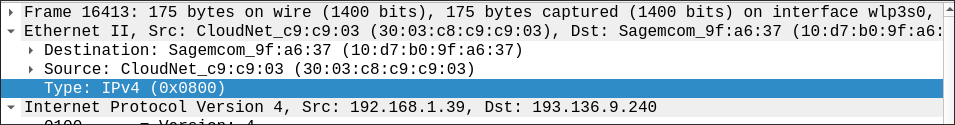
\includegraphics[width=0.8\textwidth]{type.png}
    \caption{\label{fig:type}Campo Type da trama.}
\end{figure}

\subsection{Quantos bytes são usados desde o início da trama até ao caractere ASCII “G” do
método HTTP GET? Calcule e indique, em percentagem, a sobrecarga (overhead)
introduzida pela pilha protocolar no envio do HTTP GET (considere os bytes
ocupados pela camada física e pelo FCS, indicados na Figura 1).}

\begin{figure}[h]
    \centering
    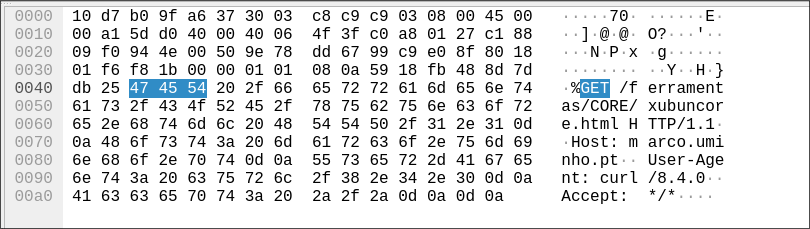
\includegraphics[width=0.8\textwidth]{byte.png}
    \caption{\label{fig:byte}Trama em formato de bytes.}
\end{figure}

\begin{figure}[h]
    \centering
    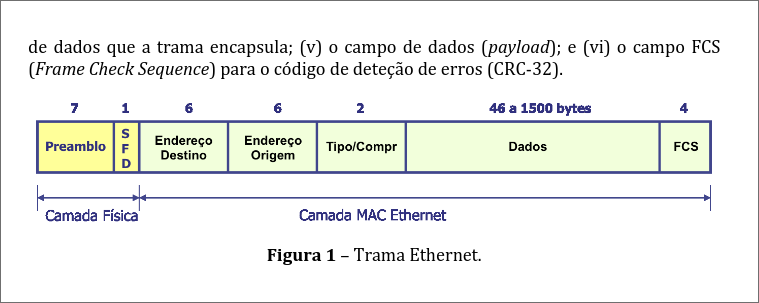
\includegraphics[width=0.8\textwidth]{fcs.png}
    \caption{\label{fig:fcs}Tamanhos do preamblo, SFD e FCS.}
\end{figure}

Observa-se que o caractere "G" está na posição 0x42 da trama = 66 bytes. Considerando que o preamblo e o SFD ocupam 7+1 bytes no inicio da trama, o numero de bytes usados desde o incio da trama ate ao caractere ASCII "G" é 66+8 = 74 bytes.

O tamanho da trama, sem o preamblo, o SFD, e o FCS é 175 bytes, com o preamblo, o SFD, e o FCS é 175+7+1+4 = 187 bytes.
O tamanho do HTTP GET é 175-66=109 bytes. Logo, a sobrecarga é de 187-109=78 bytes.
Em percentagem temos: 78/187 = 41.71\% de sobrecarga.

\subsection*{A seguir responda às seguintes perguntas, baseado no conteúdo da trama Ethernet que
contém o primeiro byte da resposta HTTP}

\begin{verbatim}
    No. Time Source Destination Protocol Length Info
    16427 13.899293562 193.136.9.240 192.168.1.39 HTTP 479 HTTP/1.1 200 OK(text/html)

    Frame 16427: 479 bytes on wire (3832 bits), 479 bytes captured (3832 bits) on interface wlp3s0, id0

    Ethernet II, Src: Sagemcom_9f:a6:37 (10:d7:b0:9f:a6:37), Dst: CloudNet_c9:c9:03
    (30:03:c8:c9:c9:03)
    Destination: CloudNet_c9:c9:03 (30:03:c8:c9:c9:03)
    Source: Sagemcom_9f:a6:37 (10:d7:b0:9f:a6:37)
    Type: IPv4 (0x0800)

    Internet Protocol Version 4, Src: 193.136.9.240, Dst: 192.168.1.39
    0100 .... = Version: 4
    .... 0101 = Header Length: 20 bytes (5)
    Differentiated Services Field: 0x00 (DSCP: CS0, ECN: Not-ECT)
    Total Length: 465
    Identification: 0xb880 (47232)
    010. .... = Flags: 0x2, Don't fragment
    ...0 0000 0000 0000 = Fragment Offset: 0
    Time to Live: 53

    Protocol: TCP (6)
    Header Checksum: 0xfe5e [validation disabled]
    [Header checksum status: Unverified]
    Source Address: 193.136.9.240
    Destination Address: 192.168.1.39
    Transmission Control Protocol, Src Port: 80, Dst Port: 37966, Seq: 8689, Ack: 110, Len: 413
    [7 Reassembled TCP Segments (9101 bytes): #16415(1448), #16417(1448), #16419(1448), #16421(1448),
    #16423(1448), #16425(1448), #16427(413)]

    Hypertext Transfer Protocol
    Line-based text data: text/html (245 lines)
\end{verbatim}

\subsection{Quais são os endereços Ethernet da origem e destino? A que sistemas de rede
correspondem? Justifique.}

Os endereços Ethernet localizam-se na camada Ethernet do modelo OSI, e são:
\begin{itemize}
    \item Endereço de origem: 10:d7:b0:9f:a6:37 (Sagemcom\_9f:a6:37 / O router) \linebreak
    O endereço de origem é o endereço do router, pois foi o router que enviou a trama.
    \item Endereço de destino: 30:03:c8:c9:c9:03 (CloudNet\_c9:c9:03 / O nosso computador) \linebreak
    O endereço de destino é o endereço do nosso computador, pois foi o nosso computador que recebeu a trama.
\end{itemize}

\subsection{Atendendo ao conceito de desencapsulamento protocolar, identifique os vários
protocolos contidos na trama recebida.}

Os protocolos contidos na trama recebida são:
\begin{itemize}
    \item Ethernet II
    \item IPv4
    \item TCP
    \item HTTP
\end{itemize}